\chapter{Results}

\section{Preparation}
\begin{figure}[h]
    \centering
    \begin{subfigure}{0.25\textwidth}
        \includegraphics[width = \textwidth]{Plots/Fe.png}
        \caption{}
        \label{fig:leed_Fe}
    \end{subfigure}
    \hfill
    \begin{subfigure}{0.25\textwidth}
        \includegraphics[width = \textwidth]{Plots/FeO.png}
        \caption{}
        \label{fig:leed_FeO}
    \end{subfigure}
    \hfill
    \begin{subfigure}{0.25\textwidth}
        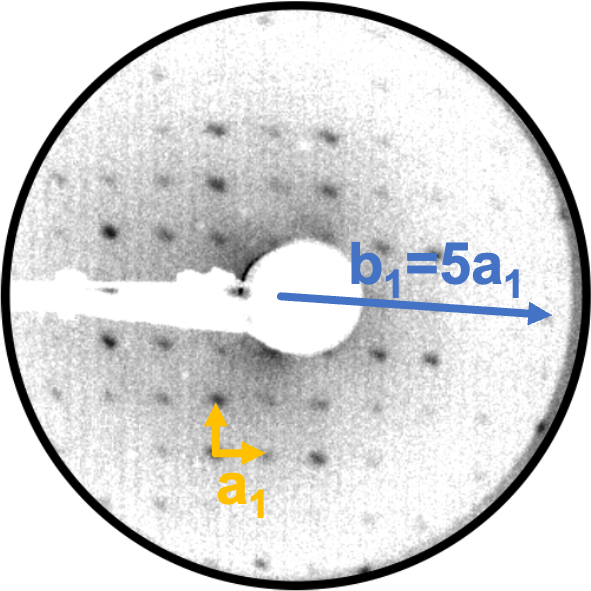
\includegraphics[width = \textwidth]{Plots/FeO_ZnTPP.png}
        \caption{}
        \label{fig:leed_FeO_ZnTPP}
    \end{subfigure}
    \caption{LEED image of the \textbf{(a)} Fe(100) surface, taken at an electron beam energy of \qty{90}{eV}, the \textbf{(b)} Fe(100)-\textit{p}(1\times1)O surface, taken at an electron beam energy of \qty{90}{eV} and \textbf{(c)} the Fe(100)-\textit{p}(1\times1)O/ZnTPP surface, taken at an electron beam energy of \qty{32}{eV}, where an ordered 1ML coverage can be deduced.}
    \label{fig:leed_1}
\end{figure}
\FloatBarrier

To confirm the quality of the Fe(100)-\textit{p}(1\times1)O surfac, a LEED image was taken before and after passivation at the same electron beam energy of \qty{90}{eV}, displayed in Figures \ref{fig:leed_Fe} and \ref{fig:leed_FeO}.
The comparison to the clean surface shows no degradation of the spot sharpness, which indicates a complete monolayer coverage without contamination.
There is also no change in spot position, so that a (1\times1) reconstruction of oxygen atoms can be confirmed.
As can be seen in \autoref{fig:leed_FeO_ZnTPP} the ZnTPP forms a commensurate square (5\times5) super-lattice, which shows a certain interaction with the substrate, not strong enough to form islands like seen on a clean Fe(100) surface \cite*{bussetti_structure_2016}, but present enough to still interact with the substrate and self-assembly in an ordered way.
The reciprocal lattice constant of the underlying substrate $a_1$ is five times the reciprocal lattice constant of the reconstruction $b_1$, meaning that the ZnTPP molecules are apart $14,25\,$\r{A}, five times the Fe lattice constant $2,85\,$\r{A} \cite*{davey_precision_1925}.

\begin{figure}[h]
    \centering
    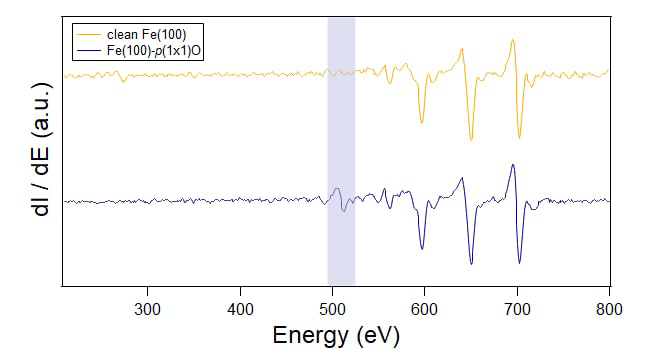
\includegraphics[width = 0.7\textwidth]{Plots/Auger.png}
    \caption{The derived intensity of the Auger spectra after cleaning the Fe(100) surface (top) and after passivation (bottom). The oxygen peak is located at \qty{503}{eV} and highlighted in the graph.}
    \label{fig:auger_FeO}
\end{figure}
\FloatBarrier
Comparing the Auger spectra of the clean and passivated Fe(100) surface also shows a significant increase in the peak at \qty{503}{eV} belonging to oxygen.
From a chemical composition point of view this poses as another confirmation, that the Fe(100) surface was successfully passivated.

For the clean Cu(100) substrate, as expected, a square lattice can be seen in \autoref{fig:leed_Cu}.
After deposition of the ZnTPP molecules on the surface, a complex LEED pattern due to several domains is visible in \autoref{fig:leed_Cu_ZnTPP}.
There could not be found a commensurate super-lattice, which would recreate this pattern, but the sharp spots clearly show an ordered assembly of the molecules on the Cu(100) substrate and indictae a 1ML coverage.
\begin{figure}[h]
    \centering
    \begin{subfigure}{0.49\textwidth}
        \centering
        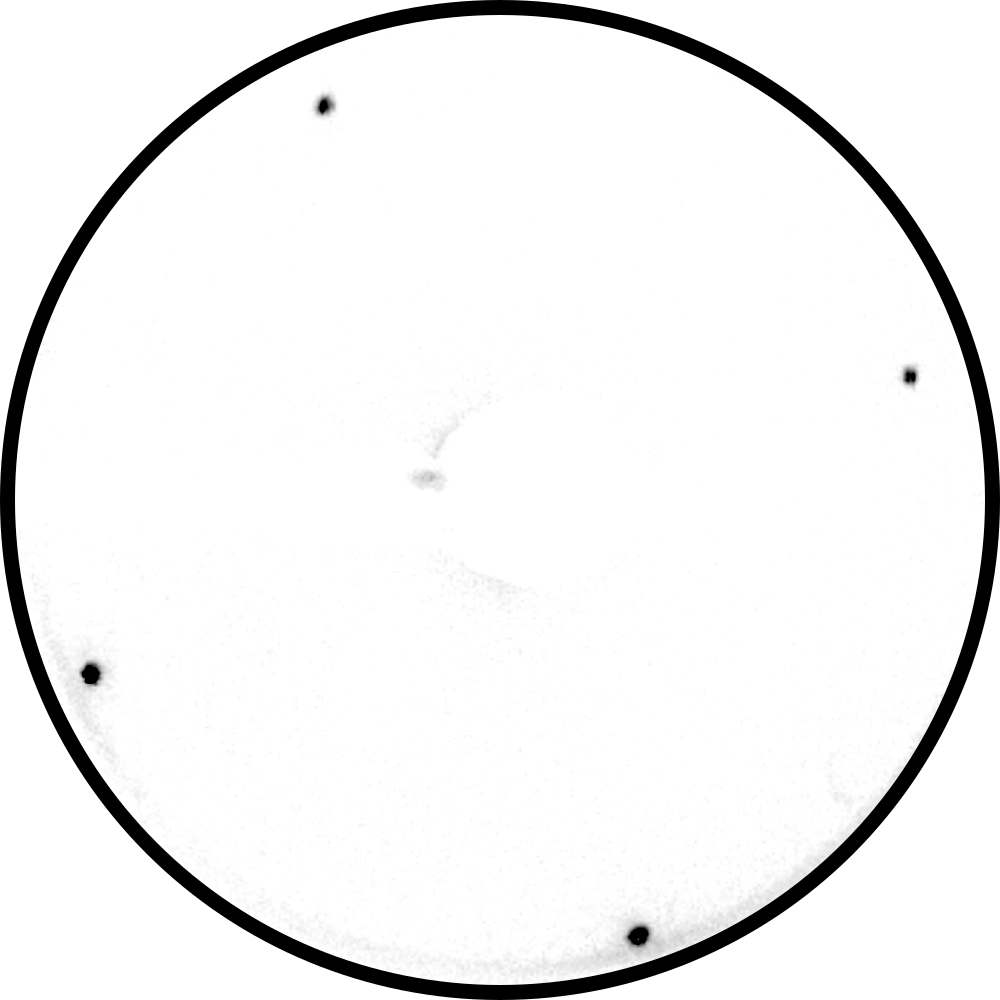
\includegraphics[width = 0.5\textwidth]{Plots/Cu.png}
        \caption{}
        \label{fig:leed_Cu}
    \end{subfigure}
    \hfill
    \begin{subfigure}{0.49\textwidth}
        \centering
        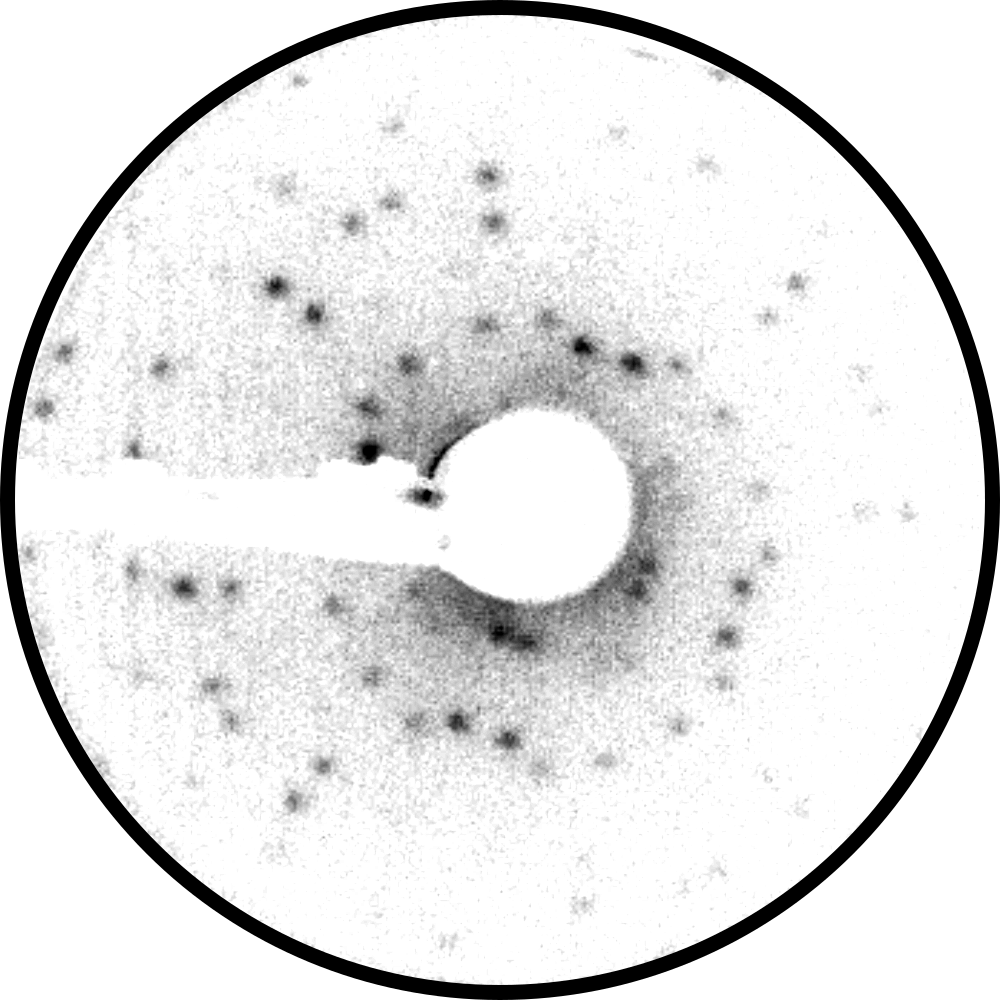
\includegraphics[width = 0.5\textwidth]{Plots/Cu_ZnTPP.png}
        \caption{}
        \label{fig:leed_Cu_ZnTPP}
    \end{subfigure}
    \caption{LEED image of the \textbf{(a)} Cu(100) surface, taken at an electron beam energy of \qty{44}{eV} and \textbf{(b)} the Cu(100)/ZnTPP surface, taken at an electron beam energy of \qty{32}{eV}.}
    \label{fig:leed_2}
\end{figure}
\FloatBarrier

\newpage
\section{Electronic structure characterization}
\begin{figure}[h]
    \centering
    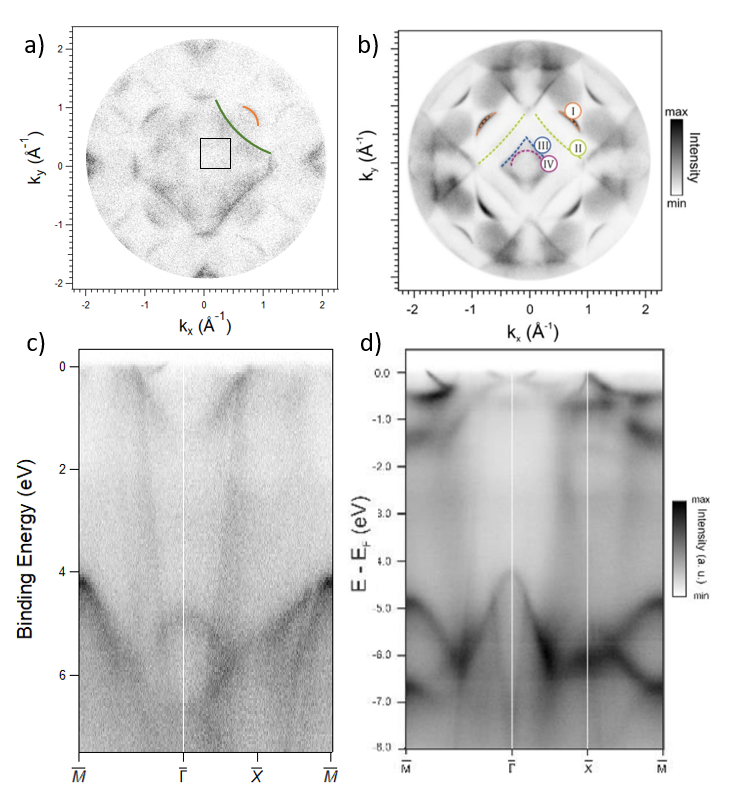
\includegraphics[width = 0.7\textwidth]{Plots/bandstructure.png}
    \caption{Momentum maps at the fermi level (top) and the bandstructure for the Fe(100)-\textit{p}(1\times1)O surface along the $\overline{M}$-$\overline{\Gamma}$-$\overline{X}$-$\overline{M}$ line (bottom). The data displayed in \textbf{(a)} and \textbf{(c)} was measured with the He lamp, \textbf{(b)} and \textbf{(d)} were taken from \cite*{janas_enhancing_2022}, where the data was aquired at a synchrotron.}
    \label{fig:bandstructure}
\end{figure}
\FloatBarrier
As reported from Janas et al. \cite*{janas_enhancing_2022} and displayed in \autoref{fig:bandstructure}b) the momentum map for the passivated Fe(100) surface at the fermi level shows distinct features numbered I to IV.
In our data \autoref{fig:bandstructure}a) we can verify the features I and II, highlighted by lines drawn in the upper right quarter of the map.
The features III and IV around the $\Gamma$ point (black square) can not be confirmed in our data.
It should be noted, that the momentum map of Janas et al. \cite*{janas_enhancing_2022} was taken at a photon energy of \qty{64}{eV}.
This corresponds to a sphere cutting the 3D bulk brillouin zone at a different energy value ($k_z$), meaning that features changing with the photon energy are related to the bulk crystal.
\autoref{fig:bandstructure}d) taken at a lower photon energy of \qty{30}{eV} contrary to \autoref{fig:bandstructure}b) taken at \qty{64}{eV} shows no strong features near the $\Gamma$ point at the fermi level upholding the before stated theory.
As can be seen in \autoref{fig:bandstructure}d) at the fermi level

Allerdings wurden die Daten bei einer Elektronenenrgie von 64eV aufgenommen \autoref{fig:bandstructure}d), wie wir sehen werden die Features bei niedrigeren Energieen weniger intensiv.

\begin{figure}[h]
    \centering
    \begin{subfigure}{0.49\textwidth}
        \centering
        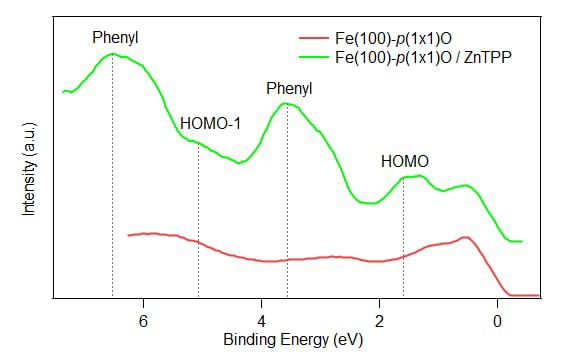
\includegraphics[width = \textwidth]{Plots/integrated_spectrum_Fe.png}
        \caption{}
        \label{fig:ups_spectrum}
    \end{subfigure}
    \hfill
    \begin{subfigure}{0.49\textwidth}
        \centering
        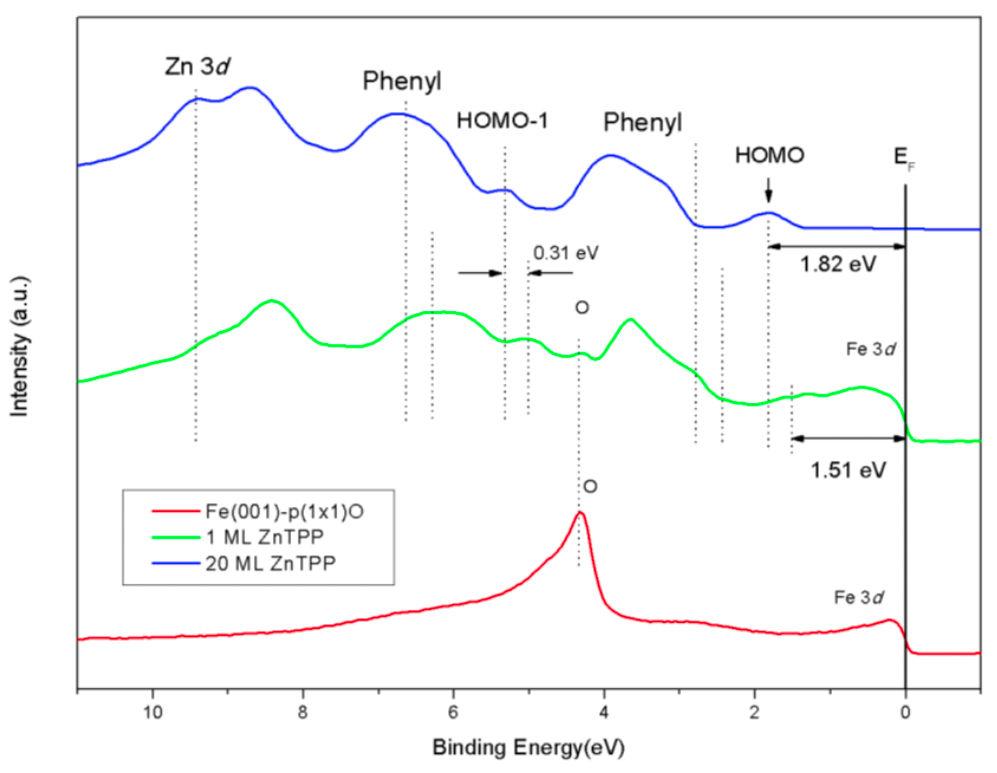
\includegraphics[width = \textwidth]{Plots/integrated_spectrum_Fe_lit.png}
        \caption{}
        \label{fig:ups_spectrum_lit}
    \end{subfigure}
    \caption{\textbf{(a)} The UPS spectrum measured for the Fe(100)-\textit{p}(1\times1)O substrate and adsorbed ZnTPP monolayer at a photon energy of $h\nu = \qty{29.8}{eV}$. \textbf{(b)} The UPS spectrum for the Fe(100)-\textit{p}(1\times1)O system taken from [...].}
    \label{fig:ups}
\end{figure}
\FloatBarrier
Using the UPS spectrum \autoref{fig:ups_spectrum_lit} taken from literature [...] the main features of our measured spectrum in \autoref{fig:ups_spectrum} could be identified.
For the red line in \autoref{fig:ups} denoting the UPS spectrum of the clean Fe(100)-\textit{p}(1\times1)O surface, a wide oxygen related peak can be discerned, although the bandstructure in \autoref{fig:bandstructure}c) shows a feature in the energy range of the oxygen peak at \qty{4.2}{eV}.
The green line corresponds to the Fe(100)-\textit{p}(1\times1)O/ZnTPP system and here the main electronic peaks can be matched to the ones from the literature.
The HOMO is measured to be at \qty{1.6}{eV} and the HOMO-1 at approximately \qty{5.1}{eV}, which coincides well with the values in \autoref{fig:ups_spectrum_lit}.
The Fe $3d$ states near the fermi level can still be observed and does not seem to have been diminished much in relation to the other features.

The UPS spectrum of Cu/ZnTPP showing no clear molecular orbitals, is not presented here, as no relevant information can be gained from it.
Because the wide UPS spectra was measured last, after the workfunction, which showed a great difference and based on this outcome it is plausible to say that the ZnTPP molecules somehow desorbed from the surface.

Now the work functions for the two samples with and without ZnTPP coverage are calculated by extrapolating the onset intersection with the energy axis. Only the difference between the work functions is important for us, because the origin of the energy axis is set by the chosen sample bias voltage.
In both cases the work function gets reduced. 
For the FeO substrate there is a shift of $\Delta\Phi_{\mathrm{FeO}} = \qty{0.31}{eV}$ and for the Cu substrate a difference in work function four times the size of $\Delta\Phi_{\mathrm{FeO}}$ can be seen $\Delta\Phi_{\mathrm{Cu}} = \qty{0.31}{eV}$.
The reduction of the sample work function can be traced back to the formation of an interface dipol through charge transfer.
Effectively the vacuum level  from the molecule to the substrate.
Meaning the 
\begin{figure}[h]
    \centering
    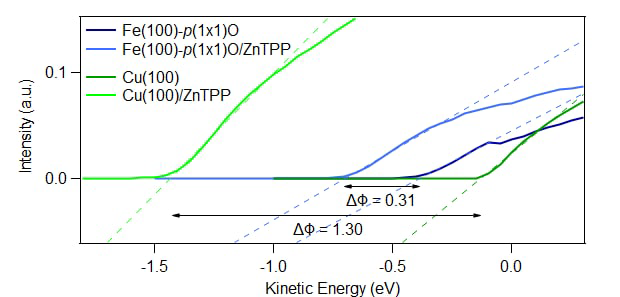
\includegraphics[width = 0.7\textwidth]{Plots/WF.png}
    \caption{Depicting the calculation of the workfunction on the UPS spectra for the Fe and Cu substrate and ZnTPP monolayers.}
    \label{fig:wf}
\end{figure}
\FloatBarrier
